\section{Implicit Q-Learning}

In this problem, you'll implement the \href{https://arxiv.org/abs/2110.06169}{Implicit Q-Learning} (IQL) method for offline RL. The actor update for IQL incorporates the advantage function similar to the actor update in the \href{https://arxiv.org/abs/2006.09359}{Advantage-Weighted Actor Critic} (AWAC) algorithm. This is an advantage-weighted negative log likelihood loss function: 
\begin{equation}
    L_\pi(\psi)=-\mathbb{E}_{s, a \sim \mathcal{B}}\left[\log \pi_\psi(a \mid s) \exp \left(\frac{1}{\lambda} \mathcal{A}^{\pi_k}(s, a)\right)\right]
\end{equation}

where $\mathcal{B}$ represents samples sampled from the dataset (behavior policy that was used to collect the data). 

The actor update in AWAC corresponds to weighted maximum likelihood, where the targets are updated by reweighting the state-action pairs observed in the current dataset by the predicted advantages from the learned critic. The Q function is learnt with a Temporal Difference (TD) loss. The objective function is given below: 

\begin{equation}\label{eq:td_objective}
    \mathbb{E}_D\left[\left(Q(s, a)- (r(s, a)+\gamma \mathbb{E}_{s^{\prime}, a^{\prime}}\left[Q_{\phi_{k-1}}\left(s^{\prime}, a^{\prime})\right)\right]\right)^2\right]
\end{equation}

IQL modifies the actor critic update to use expectile regression. The expectile $\zeta$ of a random variable $X$ is defined as:

\begin{equation}
    \arg \min _{m_\zeta} \mathbb{E}_{x \sim X}\left[L_2^\zeta\left(x-m_\zeta\right)\right]
\end{equation}

\begin{equation}
 L_2^\zeta(\mu)= |\zeta - \mathbbm{1} \{\mu \leq 0\}|    \mu^2
\end{equation}
\begin{figure}[htbp]
    \centering
    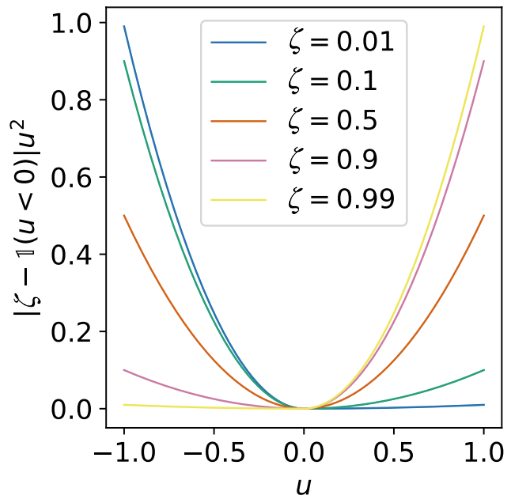
\includegraphics[scale=0.5]{figures/expectile_example.png}
    \caption{Expectile loss function visualized for different values of $\zeta$.}
    \label{fig:expectile_example}
\end{figure}

That is for $\zeta > 0.5$, this asymmetric loss function downweights the contributions of $x$ values smaller than $m_\zeta$, while giving more weights to large values as visualized in Figure \ref{fig:expectile_example}.



The offline dataset might contain different outcomes from similar states; in standard Q learning, we would want the critic to learn the expected value for any particular state-action pair. IQL, instead of learning the expected value, learns a given percentile. Our goal is to predict an upper expectile of the TD targets that approximate high values of $r(s, a) + \gamma * Q_\theta(s', a')$ which are present in the support of the offline dataset.

 

To perform this expectile regression, we need a separate parametric value function $V_{\phi}$. This allows the optimization process to be differentiable, since optimizing with a single parametric q-function implies incorporating the transition dynamics as $s' \sim p( \cdot |s, a)$. (Note the expectation over $(s', a')$ in Equation \ref{eq:td_objective}). Finally, the critic is \textbf{only} updated with actions that were seen in the offline dataset, and not on any out of distribution (unseen) sampled actions. This leads to the following loss functions:

\begin{equation}
    L_V(\phi)=\mathbb{E}_{(s, a) \sim D}\left[L_2^\zeta\left(Q_\theta(s, a)-V_\phi(s)\right)\right]
\end{equation}

\begin{equation}
    L_Q(\theta)=\mathbb{E}_{\left(s, a, s^{\prime}\right) \sim D}\left[\left(r(s, a)+\gamma V_\phi\left(s^{\prime}\right)-Q_\theta(s, a)\right)^2\right]
\end{equation}

\begin{enumerate}[(a)]

  \item \points{1a} \noindent \textbf{Implicit Q-Learning Coding} 

Implement the following functions within the below-mentioned files to finish the implementation: 

Fill in the \texttt{TODO}s in:
% ISS update
\begin{itemize}
    \item \texttt{xcs224r/critics/iql\_critic.py}
    \item \texttt{xcs224r/agents/iql\_agent.py}
\end{itemize}


  \input{01-implicit-q-learning/02-run}

  \input{01-implicit-q-learning/03-compare}

\end{enumerate}




